\documentclass{article}
% \usepackage[left=1.5cm, right=3cm, top=2cm, bottom=2cm]{geometry}
\usepackage{amsmath}
\usepackage{color}
\usepackage{framed}
\usepackage{graphicx}
\usepackage{biblatex}
\pagenumbering{gobble}
% \addbibresource{references.bib} %Import the bibliography file

\begin{document}
    \textbf{Question 4:}\\
    \textbf{Experiment}:
    Programming language: Python 3.11.3. Packages: Numpy (1.24.4), Python time module, Matplotlib (3.7.1). To implement the two algorithms, we wrote two functions $find\_triangle(n)$ and $count\_triangle(n)$. Both functions take a single input parameter, $n$, the number of vertices in the graph. The $find\_triangle(n)$ returns a boolean, True if a triangle is found, and False if no triangles. The $count\_triangle(n)$ returns an integer, zero if no triangles, or greater than zero if at least one triangle is found.\\
    \textbf{Function Summary}: \\
    Within each function call, it generates a random graph, represented as an adjacency matrix. We used a Numpy array to store an adjacency matrix with shape $(n, n)$. We used the Numpy's randomization function to fill the array elements with either 0 or 1. 1s represent edges between vertices and 0s represent no edge. Numpy's randomization function will fill the array randomly so it will not be symmetrical. Since the graph is undirected the adjacency matrix must be symmetric. Therefore to make the matrix array symmetric, we take the top diagonal half, and replace the bottom diagonal half with the transposed top half. Also, we fill the diagonal with 1s as this represents vertex self edges. \\\\
    In both algorithms, we used a nested for loop to find vertices (represented as array indices) to find rows and columns with 1s. If the element at array index $adjacency\_matrix[u][v] == 1$, there exists an edge between $(u,v)$ and $(v,u)$ since the graph is undirected. Only if a $(u,v)$ edge is found, we then used a third for loop to loop through the array indices from positions in $range(v+1, n)$ (Python range function is non-inclusive of $n$). We can start the loop at index $v+1$ because if there exists a $w$ index where $w < v$, this would have been found when $u' < u$. Similarly, we can start the $v$ for loop at index $u+1$ and we do not consider self-loops. If and only if there exists all three edges $(u,v)$ and $(u,w)$ and $(v,w)$, we have identified a triangle.\\\\
    In the $find\_triangle(n)$ algorithm, a triangle has been identified, the function terminates and returns True. If the outer for loop finishes and no vertices that satisfied the condition were found, the function returns False. Therefore, the function will terminate after the first triangle is found. In the $count\_triangle(n)$ algorithm, a counter variable, initialized to zero, is used to keep track of the number of triangles in the graph. If a triangle has been identified, the counter is incremented by a value of one. After this, the loops will continue to run until the outer loop ends. The function returns the counter variable -- the total number of triangles in the graph. \\\\
    \textbf{Experiment summary}: To calculate the average run time for each input $n$, we ran each algorithm $15$ times which used a random graph of size $n$ for each run. We used the Python time module to record the run time of the algorithm for every run and then calculated the average run time as the mean of the $15$ run times. We repeated this for each $n$. We did this for both algorithms.
    \\\\
    \textbf{Output graphs}: To generate graphs, we used Matplotlib to plot the mean run times as a line plot. The y-axis is the log2 scaled algorithm run time in seconds. The x-axis is the number of vertices, also log2 scaled.\\  
    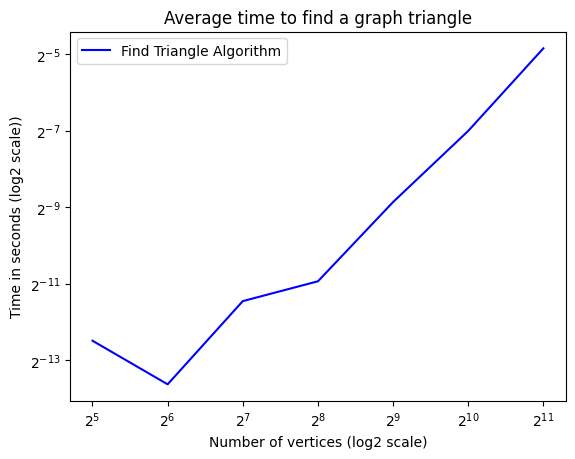
\includegraphics[width=50mm]{graph 1.png}
    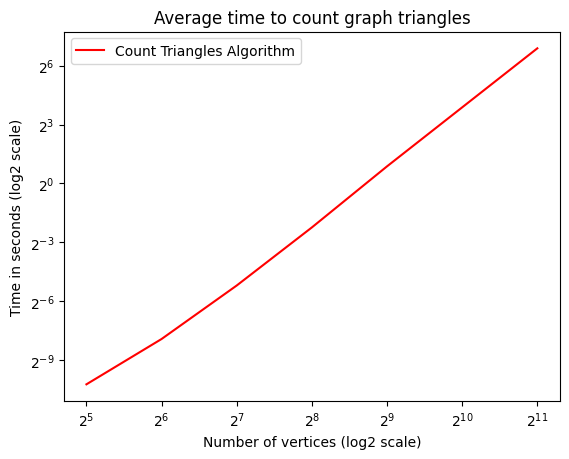
\includegraphics[width=50mm]{graph 2.png}\\
    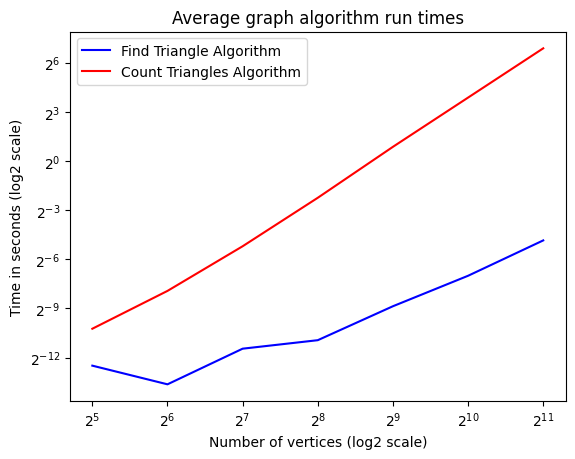
\includegraphics[width=50mm]{graph 3.png}
    \\\\
    \textbf{Conclusions}:\\
    The theoretical worst-case for the finding triangle algorithm is the worst-case run time of the counting algorithm. The counting algorithm has the same average and worst-case run times. From our experiments, the average run time of the finding algorithm was always shorter than the run time of the counting algorithm.  Looking at the finding algorithm (blue line) and the counting algorithm (red line), we can see that both algorithm run times have a positive slope increase as $n$ increases. Additionally, looking at the graph with both algorithm run times plotted, we can see that the counting algorithm has much higher run times (higher values on the y-axis). From the graphs, we can see that the average run times are closest when $n$ is small, and as $n$ increases, the difference between the algorithm run times becomes greater. From our experiments we can conclude that if there exists at least one triangle in the graph, the finding algorithm will always have a shorter run time as it will terminate sooner.  
    

\end{document}